\documentclass[12pt]{article}
\usepackage{graphicx}
\usepackage{xcolor}
\usepackage{subfigure}
\usepackage[margin=1.0in]{geometry}
\usepackage{float}
\usepackage{ulem}
\usepackage{amsmath}
\usepackage{mathtools}
\usepackage{wrapfig}
\renewcommand{\baselinestretch}{1.5}
\usepackage[utf8]{inputenc}
\author{Shivesh Pathak}
\title{Developing effective theories for the square lattice Hubbard model using density matrix downfolding}

\begin{document}
\maketitle
\begin{abstract}
A core problem of condensed matter physics is understanding how to systematically develop low-energy effective models for strongly correlated electron systems. 
We believe that a density matrix downfolding (DMD) method can be used to systematically build effective theories for such systems beginning with a high energy theory like the \textit{ab-initio} Hamiltonian H$_\text{ab}$.
We present as a preliminary result an effective theory developed using DMD which can accurately reproduce the spectra and properties of the lowest lying excitations of the CuO molecule.
As a step towards bulk strongly correlated materials, we propose developing effective theories using DMD for the simplest toy system which exhibits strongly correlated behavior: the 1-band square lattice Hubbard model at half-filling for various couplings U and temperatures T.
\end{abstract}
Committee: Lucas Wagner, ...
\pagebreak

\section{Introduction}
Systematically developing model Hamiltonians which can accurately describe the energies and properties of the lowest lying eigenstates for strongly correlated electron systems is a pressing problem in modern condensed matter physics. 

The necessity for non-perturbative, many-body models in describing the low-lying excited states of strongly correlated electron systems poses a difficult challenge when developing effective theories for real world systems.

Common approaches to building suitable model Hamiltonians for strongly correlated materials involve using single particle theories like density functional theory (DFT).

We propose using a DMD procedure to develop accurate many-body effective theories for single (SLG) and bi-layer graphene (BLG) systems as a step towards building a many-body model for twisted bilayer graphene (TBLG).


A core problem of condensed matter physics is understanding how to systematically develop low-energy effective models for strongly correlated electron systems. 
In the forefront of modern research are materials like high temperature superconductors and heavy fermion systems for which simple effective theories have not yet been found. 
For example, the cuprate family of high-Tc superconductors have an intricate phase diagram in the doping-temperature space with anti-ferromagnetic (AFM) insulating, superconducting, psuedo-gap, "bad metal", and Fermi-liquid like phases of which only the first and last are well understood.
The iron-pnictides also have superconducting domes, non-Fermi liquid like metallic phases, a spin-density-wave antiferommagnetic phase, all under various dopings and temperatures. 
Heavy-fermion materials have a purported quantum critical point between an AFM and Fermi-liquid phase which houses a superconducting dome, leading to another phase diagram for which building model Hamiltonians is very challenging. 

The fundamental barrier in writing down low-energy theories for strong correlated materials is the existence of non-perturbative interactions between various degrees of freedom - for example, lattice, spin and charge. 
Consider just the cuprate case for now, the two phases which are relatively well understood contain a singular important degree of freedom in the low-energy space. 
Near zero doping the cuprates are charge-transfer insulators with localized spin-1/2 low-energy degrees of freedom and resemble a Heisenberg antiferromagnet away from the magnetic Brillouin zone. 
In the heavily overdoped side, the lowest energy single-particle excitations look like well defined quasiparticles resembling a Fermi liquid apart from non-standard plasmonic modes. 
In the intermediate doping region where the low-energy excitations cannot be easily sectioned into spin-like or electron-like only, we see the emergence of exotic phases and where most difficulties arise in writing down low-energy effective models. 

Common approaches to building suitable model Hamiltonians for strongly correlated materials involve using single particle theories like density functional theory (DFT).
One-body terms are typically obtained by projecting the solutions from the DFT band structure onto a localized single-particle basis, giving an estimate of hoppings and occupations on a lattice model.
Two-body terms in the model are developed by assuming a screened Coulomb interaction based on constrained DFT or RPA.
Aside from this method, L\''{o}wdin methods coupled to a stochastic method and canonical transformations have also been used to develop effective theories.
These methods have the drawback that the constructed effective theory typically does not come with any estimate of the quality of the model, therefore making model validation a phenomenological task which can lead to unclear biases in the model construction.


We propose using a density matrix downfolding (DMD) procedure to develop an accurate low-energy effective theory for twisted bilayer graphene (TBLG) beginning from the \textit{ab-initio} Hamiltonian.
TBLG exhibits strong correlation effects like unconventional superconductivity and many-body insulating states for extremely small, gate-tunable, dopings near charge neutrality for certain magic twist angles.
These strong correlation effects arise from the emergence of very flat bands near the Fermi level as one approaches the magic angles.
While some DFT calculations have generated effective single particle theories, no accurate many-body model Hamiltonian for TBLG which can describe these strong electronic correlations exists.
As discussed below, DMD provides us the unique ability to generate such accurate many-body models directly from the \textit{ab-initio} Hamiltonian.

\section{Methods}
\subsection{Density Matrix Downfolding (DMD)}
We begin by defining what we mean by a low-energy effective Hamiltonian and downfolding.
Consider a Hamiltonian $\hat{H}$ defined on a Hilbert space $\mathcal{H}$.
A low-energy effective Hamiltonian is an operator $\hat{H}_\text{eff}$ which can accurately reproduce the spectra, up to a constant, and eigenstates of $\hat{H}$ on a subpsace $\mathcal{LE}$ of the Hilbert space $\mathcal{H}$.
Here $\mathcal{LE}$ is taken to be the span of the N lowest energy eigenstates of $\hat{H}$, and $\hat{H}_\text{eff}$ is a linear combination of Hermitian operators $\hat{d}_k$ with a constant energy shift $E_0$
\begin{equation}
\hat{H}_\text{eff} = \sum_{k} g_k \hat{d}_k  + E_0.
\label{eq:Heff}
\end{equation}
The objective of Hamiltonian downfolding is to construct such an $\hat{H}_\text{eff}$ given $\hat{H}, \mathcal{H}$.

The key insight of DMD is that the Hamiltonian downfolding problem can be mapped onto a linear regression problem.
It has been shown that the above definition of $\hat{H}_\text{eff}$ is equivalent to the following: a low-energy effective Hamiltonian is an operator on a subspace $\mathcal{LE}$ of $\mathcal{H}$ such that 
\begin{equation}
\begin{split}
\forall |\Psi\rangle \in \mathcal{LE},\ (E[\Psi] \equiv \langle \Psi|\hat{H} | \Psi \rangle)  = \\ (E_\text{eff}[\Psi] \equiv \langle \Psi | \hat{H}_\text{eff} | \Psi \rangle) + \epsilon[\Psi]
\end{split}
\label{eq:DMD}
\end{equation}
where $\epsilon[\Psi]$ is the error in the effective theory.
Given the general linear form of $\hat{H}_\text{eff}$ seen in \eqref{eq:Heff}, 
the task of building an effective Hamiltonian then reduces to fitting a linear model that minimizes the error $\epsilon[\Psi]$ over $\mathcal{LE}$.
The independent variables (descriptors) in the fitting are expectation values of the operators $d_k[\Psi] \equiv \langle \Psi |\hat{d}_k|\Psi \rangle$ and the target variable is $E[\Psi]$.

This linear regression problem can be tackled in three steps, beginning with sampling states from $\mathcal{LE}$.
Ideally the linear regression would be conducted over the entire space $\mathcal{LE}$. 
In practice, the space is too large, and instead a representative sample set is drawn and used for fitting.
For each sampled state $|\Psi_s\rangle$, the quantities $E[\Psi_s], \{d_k[\Psi_s]\}$ are calculated to be used in the linear regression.
Optimal sampling schemes vary between systems and can significantly reduce the number of samples required to achieve robust statistics.

Generally, however, one cannot sample the true low-energy subspace and low-energy wave functions are sampled from an approximate subspace $\mathcal{LE}^\prime$.
A model fit to an arbitrary subspace of $\mathcal{H}$ will generally fail in describing the low-energy excitations of $\hat{H}$.
Rather, the choice of approximate subspace must be made carefully to ensure the fit model is transferable to the true low-energy space.
We describe in detail later how we selected $\mathcal{LE}^\prime$ for the CuO molecule and the scheme used to draw samples from it.

Next, a set of candidate descriptors which form the effective Hamiltonian are selected.
Descriptors will typically be selected if their values co-vary with the energy over the set of sampled states. 
Knowledge of the low-energy degrees of the freedom from experiment and physical intuition can help restrict the set of candidate descriptors further.
In principle there is no restriction on the form of the candidate operators other than Hermiticity, but second quantized operators are commonly used.

Typically, candidate operators are written in second quantized form, and an appropriate single particle basis to express these operators must be constructed.
An appropriate choice of single particle basis can simplify the representation of the effective theory and typically depends on the system of interest.
Common choices include Bloch waves and molecular orbitals for delocalized basis elements or Wannier and intrinsic atomic orbitals for localized ones.
The selected single particle basis can be validated by ensuring it accurately describes single particle properties among the sampled states like the total number of electrons in the system.

Finally, the sampled data are used to fit the coefficients $\{g_k\}$ by linear regression.
A typical fitting workflow involves feature selection, model regression and model validation.
Feature selection methods for choosing appropriate descriptors can range from wrapper methods like orthogonal matching pursuit and principal component analysis to embedded methods like LASSO, ridge and elastic net regularizations. 
Fitting the effective Hamiltonian usually involves an ordinary least squares linear regression, but the cost function can be altered as in the cases of the embedded methods above or weighted least squares linear regression.
Model validation can be carried out by calculating cross validated single parameter measures like R$^2$ scores which carry information about goodness of fit and overfitting.

Importantly, the fit effective Hamiltonian carries with it a quantitative measure of its validity.
The ability to quantify the accuracy of an effective Hamiltonian sets DMD apart from contemporary downfolding approaches which typically report only a final model.
Given the statistical nature of the fitting procedure, model quality assessment can be carried out and reported in exhaustive detail if one is interested.
Typically, however, simple single parameter measures like cross validated R$^2$ scores and root mean squared errors are used to quantify the accuracy of the effective Hamiltonian.

\subsection{Fixed-node diffusion Monte Carlo (FN-DMC)}
Diffusion Monte Carlo (DMC) is a quantum Monte Carlo method which projects out the ground state of a real-space Hamiltonian given some initial trial wave function.
Consider a trial wave function $|\Psi_T\rangle$ and the Hamiltonian $\hat{H}$ with ground state $|\Phi_0\rangle$. 
Applying the projector $e^{-\tau \hat{H}}$ as $\tau \rightarrow \infty$ to $|\Psi_T \rangle$
\begin{equation}
\lim_{\tau \rightarrow \infty} e^{-\tau \hat{H}} |\Psi_T\rangle 
\equiv \lim_{\tau \rightarrow \infty} |\Psi_\text{DMC}(\tau)\rangle \propto \langle \Phi_0|\Psi_T\rangle |\Phi_0\rangle,
\end{equation}
projects out the ground state as long as the trial wave function is not orthogonal to the ground state. 
DMC provides a stochastic implementation of this projector method and involves moving samples from the trial function $\Psi_T(R)$ using the Green function $G(R, R^\prime, \tau) = \langle R | e^{-\tau(\hat{H} - E_T)} | R^\prime \rangle$. 
Since $\hat{H} = \hat{T} + \hat{V}$, kinetic and potential energy terms, the Green function is approximated by a Trotter expansion $G(R, R^\prime, \tau) = \langle R | e^{-\tau(\hat{H} - E_T)} | R^\prime \rangle \sim \Big[e^{-d\tau(\frac{V(R) + V(R^\prime)}{2} - E_T)} \langle R| e^{-d\tau\hat{T}}|R^\prime \rangle + O(d\tau^2) \Big]^N $ where $d\tau = \tau/N$.
This expansion can be interpreted as an interative procedure where samples are moved N times with a small timestep $d\tau$ until convergence.
The constant $E_T$ is a trial energy used to control the normalization of $\Psi_\text{DMC}(\tau, R)$ and is updated at each move.

DMC, however, suffers from a fermion sign problem which is alleviated via a fixed-node approximation.
Under the fixed-node approximation the nodal surface of $\Psi_\text{DMC}(\tau, R)$ is forced to match that of the initial trial wave function for all $\tau$.
This approximation makes FN-DMC variational, and will only return the exact ground state of $\hat{H}$ if the nodal surfaces of $|\Psi_T\rangle$ and $|\Phi_0\rangle$ are identical.

We take advantage of the variational nature of FN-DMC to sample the low-energy states necessary for DMD.
Consider a set of trial wave functions with varying nodal structures.
The final projected $\Psi_\text{DMC}$ for these different trial functions will be the lowest energy states in $\mathcal{H}$ for the given nodal structures.
If the initial trial wave functions are appropriately chosen, the final projected states will be low-energy states within $\Psi_\text{DMC}$.
We calculate the expectation values $E[\Psi_\text{DMC}], \{d_k[\Psi_\text{DMC}]\}$ necessary for the model regression using a mixed estimator.
Details for calculating reduced density matrix elements in FN-DMC can be found in Wagner.

\section{Preliminary Work}
\subsection{Non-orthogonal determinants in FN-DMC trial wave functions}
In order to become acquainted with our code QWalk \cite{WAGNER20093390} and QMC algorithms in general I worked on implementing and testing multi-Slater-Jastrow trial functions with optimized non-orthogonal determinants (MSJ+NO) in FN-DMC \cite{Pathak2018}.
We assessed the efficiency and compactness of this new trial function by calculating the ground state energy and single particle densities of a C$_2$ molecule using FN-DMC and comparing to the results when using multi-Slater-Jastrow trial functions with optimized orthogonal determinant trial functions (MSJ+O). 
The workflow involved constructing the un-optimized trial wave functions, optimizing the parameters using an energy optimization method \cite{Toulouse2007}, and finally using the optimized trial functions in both variational Monte Carlo (VMC) and FN-DMC calculations. 
We found the average improvement in variational energy when using optimized orthogonal determinants is $\langle E_\text{MSJ} - E_\text{MSJ+O} \rangle = $ 0.32 eV with a standard deviation of 0.08 eV, with an additional improvement from the non-orthogonal determinants of 0.031 eV with a standard deviation of 0.021 eV.
The average improvement in the FN-DMC energy with the MSJ+O trial wave functions was 0.14 eV (standard deviation 0.03 eV) with an additional reduction of 0.032 eV (standard deviation 0.019 eV) when using the MSJ+NO trial wave function.
While the benefit using the MSJ+NO trial wave function seems small, we saw that the FN-DMC energy calculated using an MSJ+NO trial function with only 24 determinants was lower than the FN-DMC energy using an MSJ+O trial function with 55 determinants.
Further, the FN-DMC charge density calculated using MSJ+NO trial functions had stronger bonding character than when using MSJ+O trial functions, a reasonable result as introducing correlations into trial functions allows for electrons to avoid each other while still occupying the same bonding region. 
Our results indicated that using non-orthogonal determinants may lead to more compact multi-Slater-Jastrow trial wave functions for small molecules.

\subsection{Effective theory for CuO molecule using DMD}
As a first step towards developing accurate models for extended systems like solids using DMD, we constructed a many-body effective model for the CuO molecule which accurately describes the eigenstates and spectra seen in experiment up to 2eV above the ground state.
The neutral CuO molecule has been a subject of intense theoretical and experimental study due to the complex structure of its low-energy space.
While the low-energy excitations in the doublet sector of the CuO molecule are well understood, singlet selection rules for spectroscopic measurements and the doublet ground state leave the quartet sector of excitations unexplored.
We construct our $\mathcal{LE}$ based on recent anion photoelectron spectroscopy (APES) measurements of the low-lying excited states of the nuetral CuO molecule. 
The lowest lying excitations involve electrons in the Cu 3d, Cu 4s and O 2p orbitals.
Given that the lowest energy excitations contain a fully-filled Cu 3d shell or a single hole in this shell we define our low-energy space as:
\begin{equation}
\mathcal{LE} = \text{Span(}\{ |\Psi \rangle | \langle \Psi | \hat{n}_{3d} | \Psi \rangle \ge 9,\ \hat{H}_\text{ab}|\Psi\rangle = E |\Psi\rangle \}\text{)}.
\label{eq:LE}
\end{equation}

Our sample space was generated by using multi-Slater-Jastrow trial wavefunctions in FN-DMC.
The parameterization for our low-energy trial wave functions was
\begin{equation}
e^{J}\sum_{i} c_i|\text{D}_i\rangle = \sum_{i} c_i (e^J |\text{D}_i \rangle) \xrightarrow{FN-DMC} \ \sim \sum_i c_i |\Phi_i \rangle \in \mathcal{LE}
\label{eq:sampling}
\end{equation}
where $e^J$ is a three-body Jastrow factor and $|\text{D}_i\rangle$ is a Slater determinant whose nodes accurately approximate those of an eigenstate $|\Phi_i \rangle \in \mathcal{LE}$.
Under the FN-DMC projection these trial wave functions map to states which are very close to linear combinations of eigenstates in $\mathcal{LE}$.
We used symmetry-targeted unrestricted Kohn-Sham (UKS) to generate our determinants $|\text{D}_i\rangle$ using a B3LYP functional, a Trail-Needs pseudopotential, and the VTZ Trail-Needs basis using the package PySCF.
This method allows us to access almost every excitation in $\mathcal{LE}$, except the few cases when two states have identical S$_z$ and number of electrons per irrep.
An example would be the ground state and the state with an excitation from Cu 3d$_{xz} \rightarrow $  O 2p$_x$, where the latter would be inaccessible.
The FN-DMC calculations were conducted with T-moves to make the calculation variational while using pseudopotentials, and a timestep of $\tau = 0.01$.
The coefficients $\{c_j\}$ for our sample states were chosen via a shell-sampling method. 
We begin by fixing the coefficient $c_0 = \sqrt{w}$ where $w \in \{1.0, 0.8,..., 0.2\}$. 
For each choice of $w$ we sample n = 5 states by randomly selecting the unassigned coefficients from a uniform distribution such that $\sum_i c_i^2 = 1$. 
We can then loop over all $i$ to generate shells of decreasing distance near each eigenstate $|\Phi_i\rangle$.

Parameterizing our effective model requires selecting a set of descriptors from which we would like to build our model and a basis on which to build our descriptors.
Occupation energies of and hybridization between Cu 3d, Cu 4s and O 2p are necessary to describe the low-energy excitations in CuO and are best represented by the occupation energies in a molecular orbital basis (MO) which would neatly package both effects.
The lack of doubly occupied Cu 4s states in the low-energy spectrum of CuO and the existence of a large Hund's coupling between the Cu 4s and 3d orbitals in the Cu atom indicate the necessity for a Hubbard U$_s$ and Hund's J$_{sd}$ respectively. 
These two interaction terms are best represented in a localized intrinsic atomic orbital (IAO).
To account for orbital relaxation between excited states in the CuO molecule we will consider including additional hybridization between MOs.
In total our space of canditate models is then 
\begin{equation}
\begin{split}
\{\bar{n}_{4s}, \bar{n}_{p_\pi}, \bar{n}_{p_z}, \hat{n}_{4s\uparrow} \hat{n}_{4s\downarrow},\sum_{i \in \{xy, xz,...\}}\vec{S}_{4s}\cdot \vec{S}_{d_i}\} \ + \\
\text{P}(\bar{c}_{d_\pi}^\dagger \bar{c}_{p_\pi} + h.c.,\ \bar{c}_{d_z^2}^\dagger \bar{c}_{p_z} + h.c.,\ \bar{c}_{4s}^\dagger \bar{c}_{p_z} + h.c.,\ \bar{c}_{d_z^2}^\dagger \bar{c}_{4s} + h.c.)
\end{split}
\label{eq:models}
\end{equation}
where P denotes the power set and operators are defined on the IAO basis unless denoted by a bar, in which case the operator is built on the MO basis. 
The coefficients for each term above will be denoted $\bar{\epsilon}_{4s},\ \bar{\epsilon}_{p_\pi},\ \bar{\epsilon}_{p_z},\ U_s,\ J_{sd},\ \bar{t}_\pi,\ \bar{t}_{dz},\ \bar{t}_{sz},\ \bar{t}_{ds}$. 
All energies will be relative to $\bar{\epsilon_{3d}} = 0$. 
The symbol $\pi$ denotes a contraction over $x, y$ for p orbitals and $xz,\ yz$ for d orbitals. The symbol $\delta$, introduced later, denotes a contraction over $xy,\ x^2-y^2$ for d orbitals.

After fitting each of the potential models in \eqref{eq:models} using ordinary least squares (OLS) linear regression we find three models which describe the energy functional on our sample set accurately with low variance, but whose eigenstates and spectra differ as a consequence of intruder states below an energy of 2eV as illustrated in Figure \ref{fig:InitED}. 
All three models have a first excited state around 1eV, but only in the minimal model does this state fall near the sample set used for the fitting.
The large distance of the eigenstates for the other two models from our sample set indicates that their predicted eigenvalues may suffer from large extrapolation errors, and as such we will call them \textit{intruder} states.
In Figure \ref{fig:Intruder} we present all eigenstates among the three potential models which we classify as intruders using a k-nearest neighbor approach with k = 5.

\begin{figure}[H]
	\centering
	\subfigure[Results of exact diagonalization showing the energies and properties of the first twenty eigenstates for three candidate models fit using ordinary linear regression. The ground state and first excited state are colored and have enlarged markers for clarity. Error bars are 95\% CI calculated by a bootstrap estimate.]{
	 	\label{fig:InitED}
		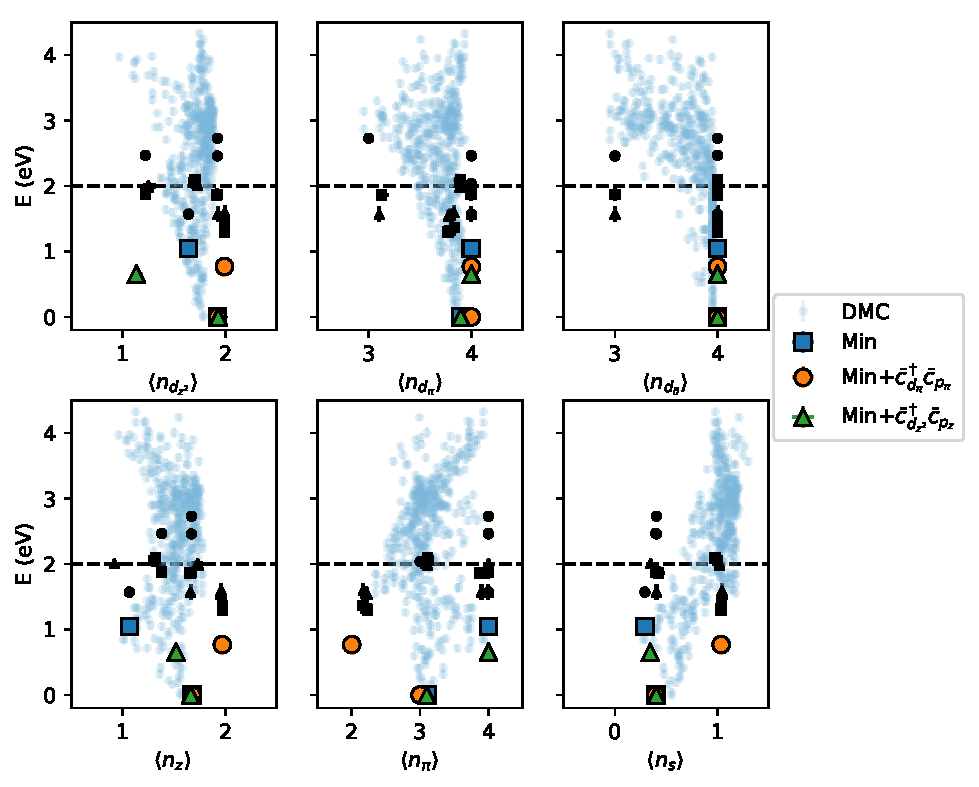
\includegraphics[width=0.45\textwidth]{figs/init_ed.pdf}
	}
	\qquad
	\subfigure[Collection of unique intruder states from our three potential models selected using a k-nearest neighbor approach with k = 5.]{	
		\label{fig:Intruder}
		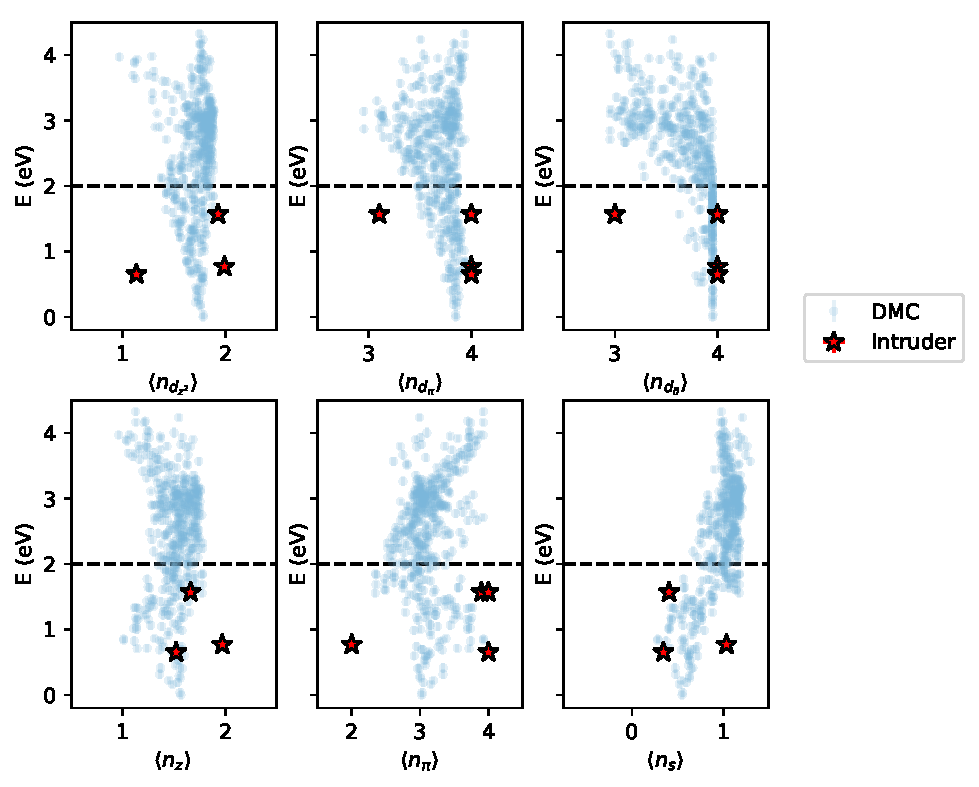
\includegraphics[width=0.45\textwidth]{figs/intruder.pdf}
	}
	\caption{Results of OLS fitting on sampled data and selected intruder states.}
\end{figure}

Given that our intruder states correspond to states within $\mathcal{LE}$ but outside our sample set, they must live within the span of the eigenstates which were excluded in our sampling scheme as described before.
This is evidenced by the fact that two of the intruder states correspond explicitly to excitations we could not access: Cu 3d$_{z^2} \rightarrow $ O 2p$_\pi$ and  Cu 3d$_\pi \rightarrow $ O 2p$_\pi$.
We can approximate these states by single rigid MO excitations above the UKS ground state, which results in states with a FN-DMC energy above 4eV.
Including a generous 2eV reduction in FN-DMC energy due to orbital relaxation, we estimate that these two states should lie at least 2eV in energy. 
Since all the other inaccessible eigenstates are double or higher order excitations, we assert a prior: intruder states should lie above 2eV in energy in our effective theories, enforced via an augmented cost function
\begin{equation}
\text{Cost} = \sum_{i} (E_\text{eff}[\Psi_i] - E_\text{ab}[\Psi_i])^2 + \lambda \sum_{p}\text{QHL}(2 - E_\text{eff}[\Psi_p]),\ \text{QHL}(x) = \Theta(x)x^2
\label{eq:cost}
\end{equation}
where $\lambda>0$ is a parameter which can be varied, QHL is a quadratic hinge loss, $\Theta$ is the Heaviside step function, the index $i$ is over our sampled states and $p$ over the selected intruder states.

\begin{figure}[H]
	\centering
	\subfigure[On the left, scores of the three candidate models at various $\lambda$ when fitting our effective theories using the cost function \eqref{eq:cost}. On the right we show predicted versus calculated energies for our low-energy sampled states for the minimal model fit at $\lambda = 20$.]{
	 	\label{fig:Prior}
		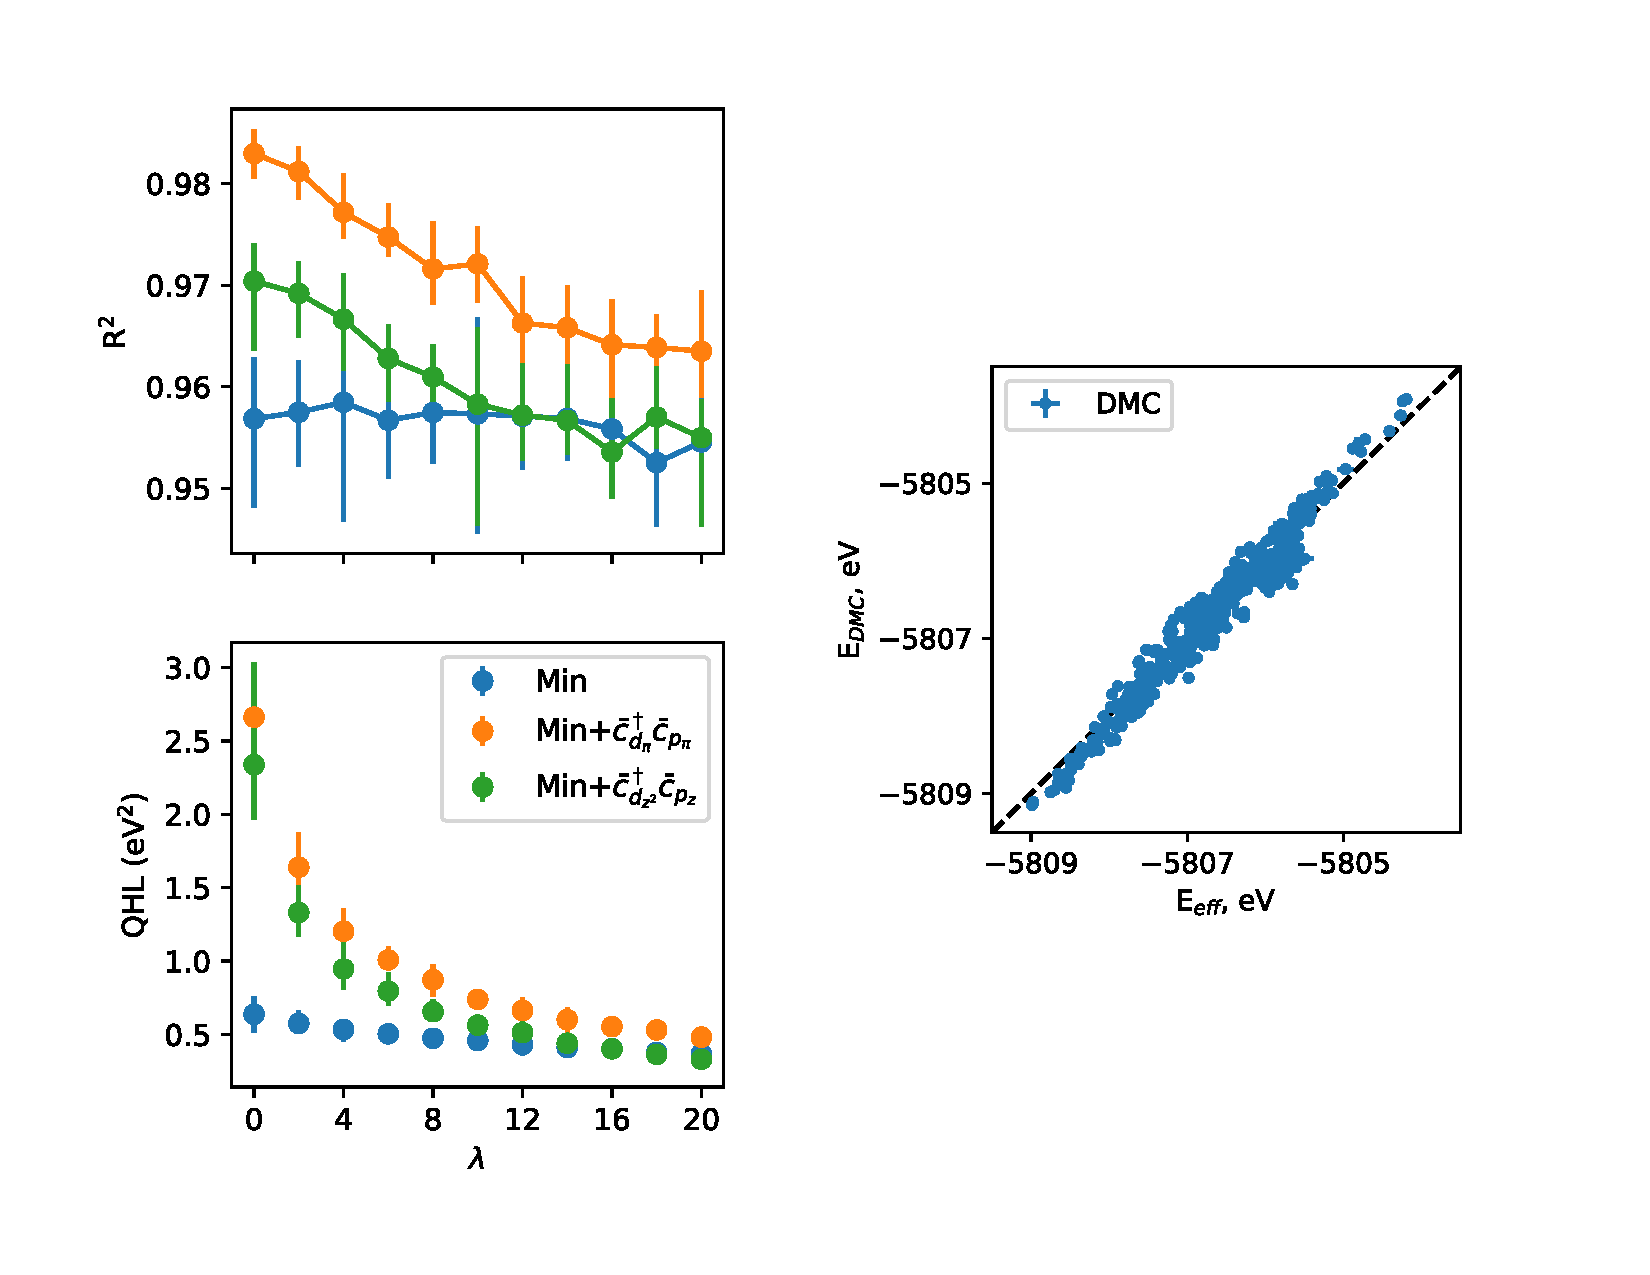
\includegraphics[width=0.45\textwidth]{figs/prior_and_regr.pdf}
	}
	\qquad
	\subfigure[Results of exact diagonalization showing the energies and properties of the first thirty eigenstates for three candidate models using linear regression with cost function \ref{eq:cost} and $\lambda = 20$. The ground state and first excited state are colored and have enlarged markers for clarity. Error bars are 95\% CI calculated by a bootstrap estimate.]{	
		\label{fig:FinalED}
		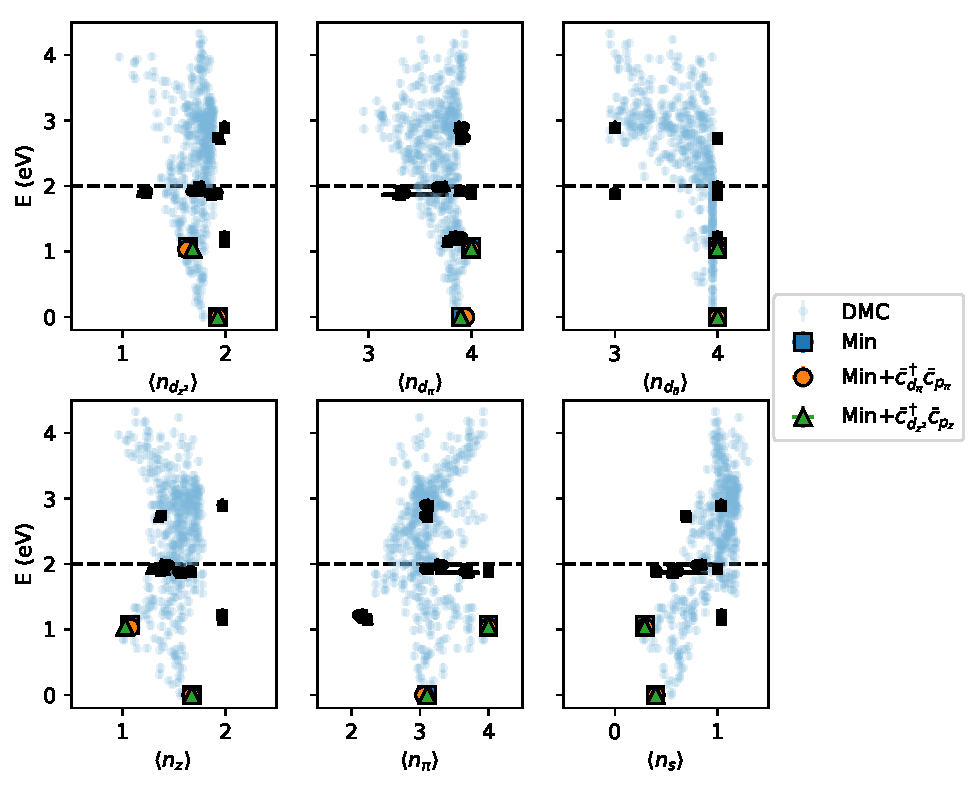
\includegraphics[width=0.45\textwidth]{figs/final_ed.pdf}
	}
	\caption{Results of linear regression using augmented cost function \eqref{eq:cost}.}
\end{figure}

Using our new cost function we find a set of models which accurately describe our sample data, have very similar spectra and eigenvectors to eachother and experiment, and do not contain intruder states below the 2eV prior. 
Shown in Figure \ref{fig:Prior} are the R$^2$ scores and QHL for the three candidate models fit at $\lambda \in [0,20]$. 
We believe that all three models at $\lambda = 20$ should be considered good models as they satisfy our prior and also explain our sample set accurately. 
Also shown are $E_\text{eff}, E_\text{ab}$ for our samples using the minimal model at $\lambda = 20$ to illustrate the high fit quality even with a large $\lambda$.
Figure \ref{fig:FinalED} presents the properties and eigenvalues of the lowest 30 eigenstates for the three fit models at $\lambda = 20$. 
The additional constraint from asserting a prior has seemingly caused a single effective theory to emerge from our set of candidate models.
This conclusion is verified by looking at the values of the fit parameters for our three models, presented in Table 1.
All occupation energies are relative to $\epsilon_{d_\delta}$.
In the doublet sector the ground and first excited state of any of the three models match experiment, as well as the block of states at 2eV corresponding to excitations out of the Cu 3d shell.
The lowest energy quartet states are at 1, 2eV respectively and are in line with the observation of a quartet state at 2eV in APES measurements.

\begin{table}[H]
\begin{center}
\begin{tabular}{l|lllll}
Model &$\epsilon_{d_{z^2}}$ & $\epsilon_{d_\pi}$ & $\epsilon_{4s}$ & $\epsilon_{p_\pi}$ & $\epsilon_{p_z}$ \\ \hline 
Min & 0.32(2)& 0.19(1)& 2.2(4)& 1.7(3)& 0.96(4)\\
Min $ +\ \bar{c}_{d_\pi}^\dagger \bar{c}_{p_\pi}$& 0.32(1)& 0.10(2)& 2.23(3)& 1.8(2)& 0.97(3)\\
Min $ +\ \bar{c}_{d_{z^2}}^\dagger \bar{c}_{p_z}$& 0.29(2)& 0.19(1)& 2.19(5)& 1.7(3)& 0.99(5)\\
\end{tabular} \\

\begin{tabular}{l|llllll}
Model &$t_\pi$ & $t_{dz}$ & $t_{sz}$ & $t_{ds}$ & $J_{sd}$ & $U_s$ \\ \hline 
Min &  -0.57(1)& 0.55(3)& 0.87(2)& 0.44(1)& -0.63(9)& 3.8(2)\\
Min $ +\ \bar{c}_{d_\pi}^\dagger \bar{c}_{p_\pi}$& -0.45(2)& 0.56(2)& 0.89(2)& 0.45(1)& -0.78(7)& 3.7(2)\\
Min $ +\ \bar{c}_{d_{z^2}}^\dagger \bar{c}_{p_z}$& -0.57(1)& 0.54(2)& 0.85(2)& 0.45(2)& -0.58(3)& 3.9(2)\\
\end{tabular} \\

\end{center}
Table 1: Parameters in eV for our three potential models when fit using \eqref{eq:cost} at $\lambda = 20$, energies relative to $\epsilon_{d_\delta} = 0$. Error bars are 95\% CI calculated using a bootstrap estimate.
\end{table}

\section{Proposed work}
My proposed plan involves building a sequence of model Hamiltonians for increasing complicated systems using DMD, working towards an accurate many-body model for TBLG.

The first system I will develop a model for is the benzene molecule.

While relatively simple, this molecule shares many similarities with and forms the basic unit of SLG.

As such, developing a model for benzene will help me become familiar with model fitting for 2-D carbon based systems.

The candidate descriptors I will use for DMD are motivated by a previous calculation on the benzene molecule.

A new constrained variational Monte Carlo (CVMC) method will be used to sample the low-energy wave functions necessary for DMD.

Note also that a model for benzene has already been developed using DMD.

This makes benzene a useful system not only for my personal learning, but as a benchmarking system for new methods like CVMC which have been developed recently.

The second system I will be interested in working on is SLG.

The model I am interested in working on will be an extension of a previous model developed for SLG using DMD.

I will extend the previous model by introducing long range density-density interactions into the effective theory.

The candidate model I anticipate to work with is an extended Hubbard model of the form.

CVMC will be used to sample the low-energy wave functions necessary to fit the model.

The last systems I will develop models for are AA and AB stacked BLG.

Being the simplest BLG configuration, these models will form a starting point for a more thorough development of models for TBLG.

I anticipate that the candidate descriptors should include interlayer couplings as well as the terms seen in SLG.

I will again use CVMC to generate the low-energy wave functions for the model regression.

The final four models can be used to investigate the transferrability of model parameters between these different carbon-based systems.

I will conclude by briefly discussing potential avenues of further study in using DMD to develop model Hamiltonians for TBLG. 

My proposed plan involves building a sequence of model Hamiltonians for increasingly complicated systems using DMD, working towards a model for TBLG.
I will begin with the basic building block of SLG, the benzene molecule, as an exercise to become familiar with the structure and chemistry of graphene like materials.
The benzene molecule consists of a hexagonal carbon ring capped by hydrogen atoms. 
It shares many features with SLG such as delocalized $\pi$ electrons and long-range charge density-density interactions.
Alongside the fact that previous DMD work has already developed an accurate model for benzene, this molecule provides a useful playground for building my familiarity with the chemistry and effective interactions in graphene like systems.

The benzene model fitting will also serve as a benchmark study for new model fitting methods developed since the first DMD calculations on it.
I will be particularly interested in testing a constrained variation Monte Carlo (CVMC) sampling method which allows us to target low-energy states with specified descriptor values.
This sampling method will be the core sampling method used in all the proposed work, with the calculations on benzene serving as an familiarizing exercise for me.
The results of my model fit using CVMC can be validated by comparing the effective theory I have built to the many-body model previous developed for benzene.

The next step will be developing a model with long range interactions for SLG, expanding on previous work.
An on-site effective Hubbard model has already been built using DMD for single-layer graphene with parameters $U/t \sim 2.00$ eV.
Following the example of the benzene molecule, however, one would expect that longer range density-density interactions would be important in describing SLG more accurately.
The goal of this step of the project would be to develop a model of the following form:
\begin{equation}
\sum_{ij} t_{ij} c_i^\dagger c_j + h.c. +  \sum_i U n_{i\uparrow} n_{i\downarrow} + \sum_{ij} V_{ij} n_i^\dagger n_j
\end{equation}
with hopping terms $t_{ij}$, an on-site Hubbard $U$, and long range density-density interaction $V_{ij}$.

The last part of my plan involves developing a model for AA and AB stacked bilayer graphene.
These stackings are the simplest forms of bilayer graphene as the supercell is much smaller than those for even moderate commensurate twist angles.
The relative shift in distance among the atoms between the AA and AB stackings will serve as a first step to understand how the interlayer coupling between graphene layers may depend on the distance between atoms in the layers.
The final model to fit for these cases would be identical to the one above, but with additional interlayer hopping terms.

The end result of my proposed project is four model Hamiltonians for the  benzene molecule, SLG, AA stacked BLG, and AB stacked BLG.
These four models will include, at least, nearest neighbor hoppings, on-site Hubbard interactions, and long range density-density interactions.
For the AA and AB stacked BLG we will also consider interlayer couplings starting with just hoppings between the layers.
Each model will come with fit parameter values, an appropriate single particle basis, and a measure of the goodness of fit for the model.
These models can be solved and compared to experiment.

With these models we can resolve an interesting question: are model parameters transferable between benzene, SLG and BLG?
The question of transferability of model parameters between SLG and BLG is quite interesting because it may inform us about how much the behavior of each graphene sheet changes once we stack them.
If the interlayer coupling does not affect the effective behavior on the single sheets, then one can easily treat the final model for bi-layer graphene in two independent pieces: an accurate model for the graphene sheets with a position dependent interlaying coupling.
However, if the interlayer coupling plays a large role in the effective theory then it may be impossible to separate the BLG model into these two pieces.
A similar study can be done for the single particle basis, giving some information about orbital relaxation going from SLG to BLG.

My work will provide a useful baseline to begin studies on TBLG.
The approach to TBLG is still very far away and will require all of the previous steps above. 
Afterwards, work on TBLG will require building effective theories of BLG with multiple twist angles, or at least varying local distances between atoms.
The goal here is to develop models for BLG where the parameters, like interlayer coupling, are defined continuously as a function of atomic distance.
The resulting interacting lattice model can then be solved over very large supercell sizes and a second step of downfolding can be done.
The goal of this second step would be to downfold the lattice model into a continuum model over the length scale of the Moire patterns seen in small twist angle BLG.
Work on TBLG would be highly exploratory, and the steps detailed here are very speculative, outlining a possible avenue of work continuing after my thesis.

\subsection{Proposed timeline}
I believe that developing effective theories for the half-filled Hubbard model should take 2 years. 
16 months should be spent on T = 0 calculations.
The first 8 months will be focused on exact diagonalization.
In this period, the first two months would be spent developing an efficient sampling scheme for $\mathcal{LE}$.
The following three months will be geared towards DMD for increasing system sizes from 2x2 to 4x4 lattices for U = 2, 12 in order to identify the existence of multiple zero temperature phases and will be primarily exploratory.
The next three months will be focused on studying intermediate U and the transition between the two phases, if they exist.
The following 8 months will be focused on finite size extrapolation.
The first two months here will be dedicated to extending our ED sampling scheme to VMC.
The following six months will involve extending our finite size results to the thermodynamic limit.
At the end of the first 16 months I should have a phase diagram at T = 0 with effective theories at various U.
The last 8 month chunk will be dedicated to the T $>$ 0 model fitting.
The first four months will be dedicated to exact diagonalization calculations and should be a relatively simple extension of the T = 0 model fitting with samples drawn according to an additional importance criteria $e^{-\beta E}$.
The last four months will be focused on extending our T = 0 VMC scheme to T $>$ 0 and conducting finite size extrapolation.
At the end of the 2 years I should have a phase diagram in the U - T space with effective theories at various values of U, T and an understanding of the phases and transitions between them.
\end{document}